\documentclass[9pt, landscape, a4paper]{article}

\usepackage{fontspec}
\renewcommand{\normalsize}{\fontsize{9}{11}\selectfont}
\usepackage[english]{babel}
\babelfont{rm}{Noto Sans}
\babelfont{sf}{Noto Sans}

\usepackage{amsmath}
\usepackage{amssymb}
\usepackage{hyperref}
\usepackage{url}
\usepackage{graphicx}
\usepackage{geometry}
\usepackage{enumitem}
\usepackage{parskip}
\usepackage{chemfig}
\usepackage{pdfpages}
\usepackage{eso-pic}
\usepackage{xcolor}
\usepackage{tikz}
\usepackage{fancybox}
\usepackage{makecell}
\usepackage{pgfplots}
\usepackage{ulem}
\usepackage{wrapfig}
\usepackage{subcaption}
\usepackage{esvect}
\usepackage{siunitx}
\usepackage{mathtools}
\usepackage{varwidth}
\usepackage{multicol}
\usepackage{titlesec}
\usepackage{bm}
\usepackage{forest}
\usepackage{upgreek}
\usepackage{tabularx}
\usepackage{booktabs}
\usepackage{colortbl}
\usepackage[column=O]{cellspace}
\usepackage{tcolorbox}
\usepackage{fancyhdr}

\usetikzlibrary{arrows, arrows.meta}
\usetikzlibrary{decorations.pathreplacing}
\usetikzlibrary{decorations.markings}
\usetikzlibrary{patterns}
\pgfplotsset{compat=1.18}

\definecolor{darkgreen}{rgb}{0.0, 0.6, 0.0}
\DeclareMathOperator\arctanh{arctanh}

% ============= TABLE COLORS =============
\definecolor{col1}{RGB}{80,60,160}
\definecolor{col2}{RGB}{40,140,60}
\definecolor{col3}{RGB}{50,80,180}
\definecolor{col4}{RGB}{200,100,0}
\definecolor{headerblue}{RGB}{220,230,245}
\definecolor{headertxt}{RGB}{40,60,120}
\definecolor{notebg}{RGB}{255,248,220}
\definecolor{noteborder}{RGB}{200,160,0}

% ============= GEOMETRY =============
\geometry{
  a4paper,
  landscape,
  left=0.5cm,
  right=0.5cm,
  top=1.5cm,
  bottom=0cm,
  footskip=0cm
}

\setlist{nosep, leftmargin=*}

\AtBeginDocument{
  \setlength{\abovedisplayskip}{3pt}
  \setlength{\belowdisplayskip}{3pt}
  \setlength{\abovedisplayshortskip}{0pt}
  \setlength{\belowdisplayshortskip}{0pt}
}

% ============= HEADER & TITLES =============
\pagestyle{fancy}
\fancyhf{}
\rhead{\small \vspace*{.1cm}Electrical Power Grid Cheatsheet}
\lhead{\small \vspace*{.1cm}Matteo Frongillo}
\cfoot{\small \thepage/10}
\renewcommand{\headrulewidth}{0pt}
\setlength{\headsep}{4pt}

\titlespacing*{\part}{0pt}{2pt}{1pt}
\titlespacing*{\section}{0pt}{2pt}{1pt}
\titlespacing*{\subsection}{0pt}{2pt}{1pt}
\titlespacing*{\subsubsection}{0pt}{1pt}{1pt}

\titleformat{\part}{\large\bfseries\color{black}}{}{0em}{}
\titleformat{\section}{\bfseries\color{red!80}}{}{0em}{}
\titleformat{\subsection}{\small\bfseries\color[HTML]{007AFF}}{}{0em}{}
\titleformat{\subsubsection}{\small\bfseries\color[HTML]{007355}}{}{0em}{}

% ============= META DATA =============
\newcommand{\pdftitle}[1]{\hypersetup{
  colorlinks=true,
  linkcolor=black,
  urlcolor=blue,
  pdftitle={#1},
  pdfauthor={Matteo Frongillo}
}}

% ============= RENEW COMMANDS =============
\makeatletter
\renewcommand{\author}[1]{%
  \def\@author{%
    #1\\
    \parbox{\textwidth}{%
      \centering
      \small Last update: \today
    }
  }%
}
\makeatother

\let\emptyset\varnothing

\makeatletter
\pgfmathdeclarefunction{arctan}{1}{%
  \begingroup
  \pgfmathparse{rad(atan(#1))}%
  \endgroup
}
\makeatother

\renewcommand{\tau}{\uptau}
\renewcommand{\nu}{\upnu}
\let\mathto\to
\renewcommand{\to}{\ensuremath{\mathto}\ }

% ============= NEW COMMANDS =============
\newtcolorbox{exercisebox}[1][Exercise]{
  colback=gray!5,
  colframe=gray!75!black,
  coltitle=white,
  colbacktitle=gray!75!black,
  title={\footnotesize\textbf{#1}},
  fontupper=\footnotesize,
  boxrule=0.6pt,
  arc=2pt,
  left=4pt,
  right=4pt,
  top=3pt,
  bottom=3pt
}

\newcommand{\figbox}[1]{
  \begin{center}
    \fbox{\begin{varwidth}{\textwidth} #1 \end{varwidth}}
  \end{center}
}

\newcommand{\wrapfill}{
  \par
  \ifnum \value{WF@wrappedlines} > 0
    \addtocounter{WF@wrappedlines}{-1}%
    \null\vspace{
      \arabic{WF@wrappedlines}
      \baselineskip
    }
    \WFclear
  \fi
  \phantom{}
}

\ExplSyntaxOn
\DeclareDocumentCommand{\integral}{d[] d[] d[] d[]}
{
  \IfNoValueTF{#3}{
    \IfNoValueTF{#4}{
      \displaystyle \int #1\,d#2
    }{
      \text{Error: either 2 or 4 arguments must be provided}
    }
  }{
    \IfNoValueTF{#4}{
      \text{Error: either 2 or 4 arguments must be provided}
    }{
      \displaystyle
      \int\limits
      \IfNoValueF{#1}{\c_math_subscript_token{#1}}
      ^{\IfNoValueTF{#2}{}{#2}}
      #3\, d#4
    }
  }
}
\ExplSyntaxOff

\newcommand*\circled[1]{\tikz[baseline=(char.base)]{
  \node[shape=circle,draw,inner sep=1pt] (char) {\small #1};}}

\makeatletter
\newcommand*{\rom}[1]{\expandafter\@slowromancap\romannumeral #1@}
\makeatother

\makeatletter
\newcommand{\shorteq}{\mathrel{\mkern0.2mu\mathpalette\shorteq@\relax\mkern0.2mu}}
\newcommand{\shorteq@}[2]{\scalebox{0.5}[1]{$\m@th#1=$}}

\newcommand{\longeq}[1]{\mathrel{\mathpalette\longeq@{#1}}}
\newcommand{\longeq@}[2]{%
  \begingroup
  \sbox\z@{$\m@th#1=$}%
  \ifdim#2<\wd\z@
    \resizebox{#2}{\height}{\box\z@}%
  \else
    \ifdim#2<3\wd\z@
      \hbox to #2{$\m@th#1=\hss=\hss=\hss=$}%
    \else
      \hbox to #2{$\m@th#1=\cleaders\hbox to 0.2\wd\z@{\hss$#1=$\hss}\hfil=$}%
    \fi
  \fi
  \endgroup
}
\makeatother

\newcommand{\const}{%
  \ \mathrel{\ooalign{%
    \hfil$c$\hfil\cr
    \hfil\kern0.10em\raisebox{-0.4ex}{\rule{0.08pt}{1.7ex}}\hfil\cr
  }}%
}

\makeatletter
\define@key{Gin}{lw}[1]{\setkeys{Gin}{width=#1\linewidth}}
\newcommand{\lw}{lw}
\makeatother

\newcommand{\difference}{\,\backslash\,}
\newcommand{\rem}{\underline{Remark}: }
\newcommand{\nots}{\underline{Notation}: }
\newcommand{\note}{\underline{Note}: }
\newcommand{\prf}{\underline{Proof}: }
\newcommand{\exs}{\underline{Example}: }
\newcommand{\defs}{\underline{Definition}: }
\newcommand{\wrn}{\underline{Warning}: }
\newcommand{\sht}{\ |\ }
\newcommand{\pph}[1]{\paragraph{#1} \phantom{}\\}
\newcommand{\dm}{\displaystyle}
\newcommand{\rad}{^{\mathrm{c}}}
\newcommand{\dsum}[2]{\displaystyle \sum_{#1}^{#2}}
\newcommand{\dx}[2]{\dfrac{{\mathrm{d}}^{#1}{#2}}{\mathrm{d}x^{#1}}}
\newcommand{\der}[2]{\dfrac{{\mathrm{d}}{#1}}{\mathrm{d}{#2}}}
\newcommand{\cel}{\ensuremath{^\circ}C}
\newcommand{\todo}{{\color{red}TODO}}
\newcommand{\hr}{\vspace{0.1cm}\par\vspace{-.5\ht\strutbox}\noindent\rule{\linewidth}{.5pt}\par\vspace{0.1cm}}

\DeclareMathOperator{\rot}{rot}

% ============= DOCUMENT CONTENT =============
\begin{document}
\pdftitle{Electrical Power Grid}

\setlength{\columnsep}{0.5cm}
\begin{multicols*}{3}
\raggedcolumns

\part{Exercises}

\section{Exercise 1: Power-flow sign convention}
\subsection{Exercise}
\begin{center}
  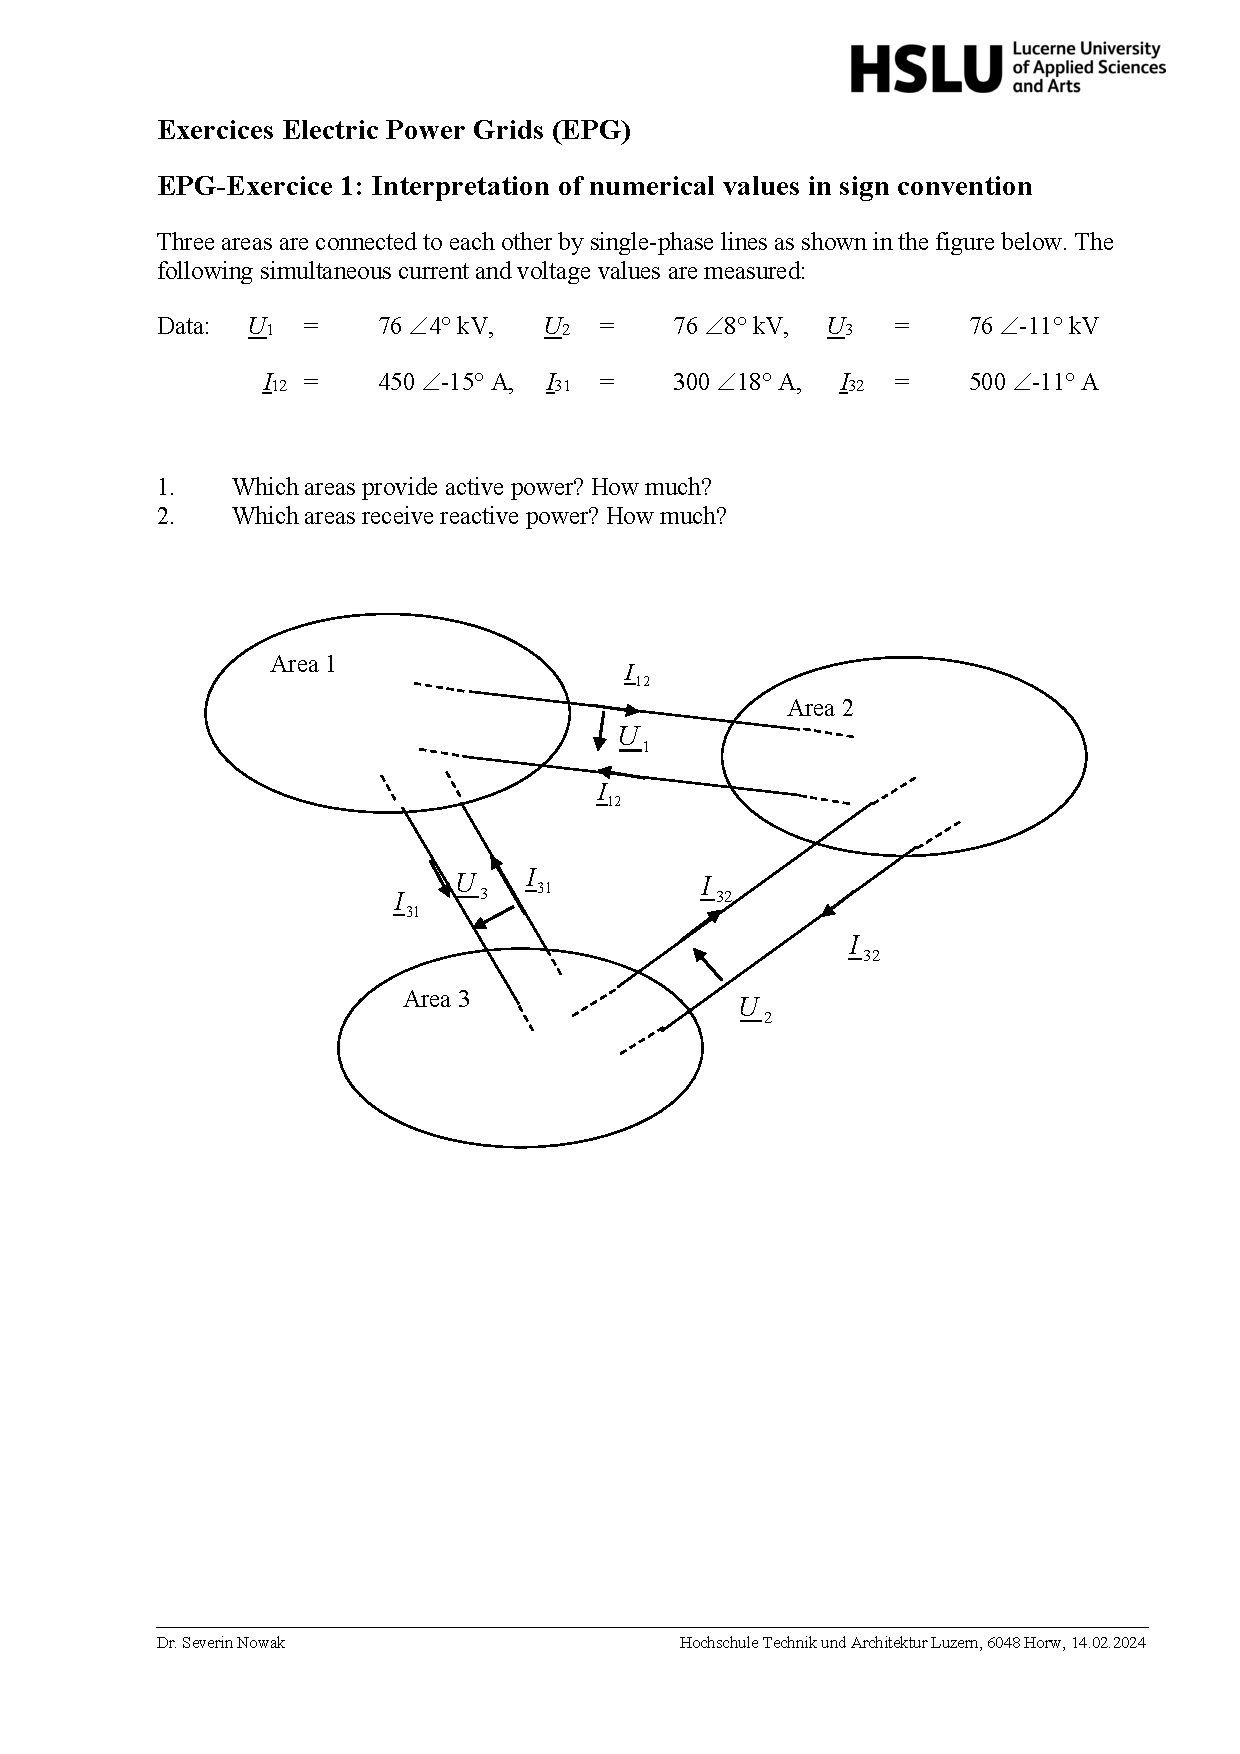
\includegraphics[page=1,width=\columnwidth,trim=1.2cm 8.4cm 1.2cm 1.3cm,clip]
  {media/Exercices_EPG_SN (1).pdf}
\end{center}

\subsection{Formulas needed}
With the reference directions shown in the exercise:
\[
  \underline S=\underline U\,\underline I^*,
  \qquad
  P=\Re\{\underline S\},
  \qquad
  Q=\Im\{\underline S\}.
\]
For phasors,
\[
  (A\angle\alpha)(B\angle\beta)^*
  =AB\angle(\alpha-\beta).
\]
Positive $P$ or $Q$ means that the area supplies active or reactive
power according to the indicated current references; a negative result
means that it receives power.

\subsection{Complete solution}
\subsubsection{Area 1}
Apply the indicated voltage and current references at the two
connections of area 1:
\begin{align*}
\underline S_1
 &=\underline U_1\underline I_{12}^*
   -\underline U_3\underline I_{31}^*\\
 &=76\angle4^\circ\cdot450\angle15^\circ\\
 &\quad-76\angle(-11^\circ)\cdot300\angle(-18^\circ)
   \ \text{MVA}/1000\\
 &=34.2\angle19^\circ-22.8\angle(-29^\circ)\\
 &=\boxed{12.40+j22.19\ \text{MVA}}.
\end{align*}
Therefore area 1 supplies $12.40$ MW and $22.19$ Mvar.

\subsubsection{Area 2}
\begin{align*}
\underline S_2
 &=\underline U_2\underline I_{32}^*
   -\underline U_1\underline I_{12}^*\\
 &=76\angle8^\circ\cdot500\angle11^\circ\\
 &\quad-76\angle4^\circ\cdot450\angle15^\circ
   \ \text{MVA}/1000\\
 &=38.0\angle19^\circ-34.2\angle19^\circ\\
 &=\boxed{3.59+j1.24\ \text{MVA}}.
\end{align*}
Area 2 supplies $3.59$ MW and $1.24$ Mvar.

\subsubsection{Area 3}
\begin{align*}
\underline S_3
 &=\underline U_3\underline I_{31}^*
   -\underline U_2\underline I_{32}^*\\
 &=76\angle(-11^\circ)\cdot300\angle(-18^\circ)\\
 &\quad-76\angle8^\circ\cdot500\angle11^\circ
   \ \text{MVA}/1000\\
 &=22.8\angle(-29^\circ)-38.0\angle19^\circ\\
 &=\boxed{-15.99-j23.43\ \text{MVA}}.
\end{align*}
Area 3 receives $15.99$ MW and $23.43$ Mvar. The check
$\underline S_1+\underline S_2+\underline S_3\simeq0$ confirms the
lossless power balance.

\section{Exercise 2: Merit-order pricing}
\subsection{Exercise}
\begin{center}
  \includegraphics[page=4,width=\columnwidth,trim=1.2cm 13.2cm 1.2cm 1.3cm,clip]
  {media/Exercices_EPG_SN (1).pdf}
\end{center}

\subsection{Formulas needed}
The supply curve is built by accumulating seller quantities from the
lowest to the highest offer price. The demand curve is accumulated from
the highest to the lowest willingness to pay. The market-clearing point
is their intersection. All accepted offers are settled at the clearing
price.

\subsection{Complete solution}
The cumulative supply is
\[
\begin{array}{c|ccccc}
p\,[\mathrm{CHF/kWh}]&.070&.075&.085&.095&.150\\
\hline
E_S\,[\mathrm{MWh}]&50&250&500&750&1150
\end{array}
\]
and the cumulative demand is
\[
\begin{array}{c|rrrrrr}
p\,[\mathrm{CHF/kWh}]&.130&.120&.110&.100&.090&.080\\
\hline
E_D\,[\mathrm{MWh}]&150&300&550&800&1000&1100.
\end{array}
\]
At $0.095$ CHF/kWh the sellers offer $750$ MWh, while demand is still
at least $800$ MWh. The next seller asks $0.15$ CHF/kWh, which is above
the next accepted demand bid. Hence
\[
  \boxed{p_\mathrm{clear}=0.10\ \mathrm{CHF/kWh}},
  \qquad
  \boxed{E_\mathrm{clear}=750\ \mathrm{MWh}}.
\]
Sellers S1--S4 are fully accepted. Buyers B4--B6 take $550$ MWh in
total, and B3 is partially accepted for the remaining $200$ MWh.
S5, B1 and B2 are not accepted.

\section{Exercise 3: Three-phase complex power}
\subsection{Exercise}
\begin{center}
  \includegraphics[page=4,width=\columnwidth,trim=1.2cm 1.8cm 1.2cm 13.0cm,clip]
  {media/Exercices_EPG_SN (1).pdf}
\end{center}

\subsection{Formulas needed}
For each delta branch:
\[
 \underline U_{ij}=\underline U_{iN}-\underline U_{jN},
 \quad
 \underline I_{ij}=\frac{\underline U_{ij}}{\underline Z_\Delta},
 \quad
 \underline S_{ij}=\underline U_{ij}\underline I_{ij}^*.
\]
The total power and power factor are
\[
 \underline S=\sum\underline S_{ij}=P+jQ,
 \qquad
 \lambda=\frac{P}{|\underline S|}=\cos\varphi.
\]

\subsection{Complete solution}
The three line-to-line voltages are
\begin{align*}
\underline U_{12}
 &=110\angle0^\circ-230\angle(-120^\circ)
  =300.50\angle41.52^\circ\ \mathrm V,\\
\underline U_{23}
 &=230\angle(-120^\circ)-230\angle120^\circ
  =398.37\angle(-90^\circ)\ \mathrm V,\\
\underline U_{31}
 &=230\angle120^\circ-110\angle0^\circ
  =300.50\angle138.48^\circ\ \mathrm V.
\end{align*}
Since $\underline Z_\Delta=30+j25=39.05\angle39.81^\circ\ \Omega$,
\begin{align*}
\underline I_{12}&=7.69\angle1.71^\circ\ \mathrm A,\\
\underline I_{23}&=10.20\angle(-129.81^\circ)\ \mathrm A,\\
\underline I_{31}&=7.69\angle98.67^\circ\ \mathrm A.
\end{align*}
Alternatively, for every branch
$\underline S_{ij}=|\underline U_{ij}|^2/\underline Z_\Delta^*$.
Adding the three branch powers gives
\[
 \underline S
 =\frac{300.50^2+398.37^2+300.50^2}{30-j25}
 =\boxed{6.675+j5.562\ \mathrm{kVA}}.
\]
Thus
\[
 |\underline S|=8.689\ \mathrm{kVA},
 \qquad
 \boxed{\lambda=6.675/8.689=0.768}.
\]
Because $Q>0$, the load is inductive and the power factor is lagging.

\section{Exercise 4: Unbalanced four-wire system}
\subsection{Exercise}
\begin{center}
  \includegraphics[page=7,width=\columnwidth,trim=1.2cm 6.4cm 1.2cm 1.3cm,clip]
  {media/Exercices_EPG_SN (1).pdf}
\end{center}

\subsection{Formulas needed}
Use nodal analysis at the floating load star point K:
\[
\underline U_{KN}
=\frac{
Y_R\underline U_{1N}+Y_L\underline U_{2N}+Y_C\underline U_{3N}}
{Y_R+Y_L+Y_C+Y_N}.
\]
Then
\[
\underline U_{iK}=\underline U_{iN}-\underline U_{KN},
\quad
\underline I_i=Y_i\underline U_{iK},
\quad
\underline I_N=Y_N\underline U_{KN}.
\]

\subsection{Complete solution}
At $\omega=2\pi50=314.16$ rad/s:
\begin{align*}
Y_R&=\frac1{100}=0.0100\ \mathrm S,\\
Y_L&=\frac1{j\omega L}=-j0.019894\ \mathrm S,\\
Y_C&=j\omega C=j0.012566\ \mathrm S,\\
Y_N&=\frac1{j\omega L_N}=-j0.006366\ \mathrm S.
\end{align*}
Substitution into the node equation gives
\[
\underline U_{KN}
=-176.97-j161.74
=\boxed{239.75\angle(-137.57^\circ)\ \mathrm V}.
\]
The load voltages are
\begin{align*}
\underline U_{1K}
 &=220\angle0^\circ-\underline U_{KN}
 =\boxed{428.66\angle22.17^\circ\ \mathrm V},\\
\underline U_{2K}
 &=220\angle(-120^\circ)-\underline U_{KN}
 =\boxed{72.90\angle(-23.26^\circ)\ \mathrm V},\\
\underline U_{3K}
 &=220\angle120^\circ-\underline U_{KN}
 =\boxed{358.57\angle79.24^\circ\ \mathrm V}.
\end{align*}
Consequently,
\begin{align*}
\underline I_1&=Y_R\underline U_{1K}
 =\boxed{4.287\angle22.17^\circ\ \mathrm A},\\
\underline I_2&=Y_L\underline U_{2K}
 =\boxed{1.450\angle(-113.26^\circ)\ \mathrm A},\\
\underline I_3&=Y_C\underline U_{3K}
 =\boxed{4.506\angle169.24^\circ\ \mathrm A},\\
\underline I_N&=Y_N\underline U_{KN}
 =\boxed{1.526\angle132.43^\circ\ \mathrm A}.
\end{align*}
The KCL check is
$\underline I_1+\underline I_2+\underline I_3=\underline I_N$.

\section{Exercise 5: Balanced three-phase system}
\subsection{Exercise}
\begin{center}
  \includegraphics[page=10,width=\columnwidth,trim=1.2cm 5.3cm 1.2cm 1.3cm,clip]
  {media/Exercices_EPG_SN (1).pdf}
\end{center}

\subsection{Formulas needed}
For a balanced system, convert the delta load to star:
\[
 \underline Z_Y=\frac{\underline Z_\Delta}{3},
 \qquad
 U_\mathrm{ph}=\frac{U_{LL}}{\sqrt3}.
\]
One phase can then be solved using
\[
 \underline I_L=\frac{\underline U_\mathrm{ph}}
 {\underline Z_\mathrm{Ltg}+\underline Z_Y},
 \qquad
 \underline U_{Y}=\underline I_L\underline Z_Y,
 \qquad
 U_\Delta=\sqrt3\,U_Y.
\]
For a star-connected capacitor bank,
\[
Y_C=j\omega C_K,\qquad
\Im\{Y_Y+Y_C\}=0.
\]

\subsection{Complete solution}
\subsubsection{a) Capacitor bank disconnected}
\[
\underline Z_Y=\frac{30\angle60^\circ}{3}
=10\angle60^\circ=5+j8.660\ \Omega,
\quad
U_\mathrm{ph}=400/\sqrt3=230.94\ \mathrm V.
\]
The per-phase total impedance is
\[
\underline Z_\mathrm{tot}
=(1+j2)+(5+j8.660)
=6+j10.660
=12.233\angle60.63^\circ\ \Omega.
\]
Taking $\underline U_{1N}=230.94\angle0^\circ$ V,
\[
\underline I_1
=\frac{230.94\angle0^\circ}{12.233\angle60.63^\circ}
=\boxed{18.879\angle(-60.63^\circ)\ \mathrm A}.
\]
The other line currents are displaced by $-120^\circ$ and $+120^\circ$:
\[
\underline I_2=18.879\angle179.37^\circ\ \mathrm A,\qquad
\underline I_3=18.879\angle59.37^\circ\ \mathrm A.
\]
The equivalent star-load phase voltage is
\[
\underline U_Y=\underline I_1\underline Z_Y
=188.79\angle(-0.63^\circ)\ \mathrm V.
\]
Therefore the magnitude across every delta branch is
\[
\boxed{U_\Delta=\sqrt3\,188.79=326.99\ \mathrm V}.
\]
For example,
$\underline U_{12,\Delta}=326.99\angle29.37^\circ$ V; the other two
delta voltages are shifted by $\mp120^\circ$. The load remains
$\boxed{\underline Z_\Delta=30\angle60^\circ\ \Omega}$ per branch.

\subsubsection{b) Reactive-current compensation}
The star-equivalent load admittance is
\[
\underline Y_Y=\frac1{5+j8.660}
=0.0500-j0.086603\ \mathrm S.
\]
The capacitor must provide $+j0.086603$ S per phase:
\[
\omega C_K=0.086603
\quad\Longrightarrow\quad
\boxed{C_K=\frac{0.086603}{2\pi50}
=275.7\ \upmu\mathrm F}
\]
per star-connected capacitor.

\subsubsection{c) Compensated line current}
The compensated parallel load has
\[
\underline Y_\mathrm{load,comp}=0.0500\ \mathrm S,
\qquad
\underline Z_\mathrm{load,comp}=20.0\ \Omega.
\]
Including the line impedance,
\[
\underline Z_\mathrm{tot,comp}=21+j2
=21.095\angle5.44^\circ\ \Omega.
\]
Hence
\[
\boxed{\underline I_1
=10.948\angle(-5.44^\circ)\ \mathrm A}.
\]
Again, $\underline I_2$ and $\underline I_3$ are shifted by
$-120^\circ$ and $+120^\circ$. Compensation reduces the current from
$18.88$ A to $10.95$ A and leaves only the line-reactance phase shift.

\section{Exercise 6: Surge impedance loading}
\subsection{Exercise}
\begin{center}
  \includegraphics[page=12,width=\columnwidth,trim=1.2cm 14.0cm 1.2cm 1.3cm,clip]
  {media/Exercices_EPG_SN (1).pdf}
\end{center}

\subsection{Formulas needed}
For a lossless line, the surge or characteristic impedance is
\[
 Z_c=\sqrt{\frac{L_b'}{C_b'}}
     =\sqrt{\frac{L_b}{C_b}}.
\]
At surge-impedance loading, the inductive and capacitive reactive
powers cancel and the resistive load is $R_L=Z_c$.

\subsection{Complete solution}
The total per-phase parameters are
\[
L_b=L_b'l=1.3\ \frac{\mathrm{mH}}{\mathrm{km}}\cdot250\ \mathrm{km}
=0.325\ \mathrm H,
\]
\[
C_b=C_b'l=9.6\ \frac{\mathrm{nF}}{\mathrm{km}}\cdot250\ \mathrm{km}
=2.40\ \upmu\mathrm F.
\]
Thus
\[
R_L=Z_c
=\sqrt{\frac{0.325}{2.40\cdot10^{-6}}}
=\boxed{367.99\ \Omega\approx368\ \Omega}.
\]
The line length cancels if the distributed values $L_b'$ and $C_b'$
are inserted directly.

\section{Exercise 7: Transformer clock number}
\subsection{Exercise}
\begin{center}
  \includegraphics[page=12,width=\columnwidth,trim=1.2cm 1.8cm 1.2cm 13.2cm,clip]
  {media/Exercices_EPG_SN (1).pdf}
\end{center}

\subsection{Formulas needed}
Transformer clock numbers add along a cascade and are evaluated modulo
12:
\[
 n_\mathrm{path}=(n_1+n_2+\cdots)\bmod12.
\]
Two paths connected to the same buses must produce the same total phase
shift.

\subsection{Complete solution}
From the 220-kV bus to the 6-kV bus, the upper path contains T5 and T4:
\[
n_\mathrm{upper}=(5+6)\bmod12=11.
\]
The lower path contains T1, T2 and T3:
\[
n_\mathrm{lower}=(6+6+n_3)\bmod12=n_3.
\]
The two paths are connected in parallel at their start and end buses,
so their phase shifts must be identical:
\[
n_3=11.
\]
Since the winding configuration is already specified as Yd,
\[
\boxed{\mathrm{T3:Yd11}}.
\]

\section{Exercise 8: Suitable transformer group}
\subsection{Exercise}
\begin{center}
  \includegraphics[page=13,width=\columnwidth,trim=1.2cm 15.3cm 1.2cm 1.3cm,clip]
  {media/Exercices_EPG_SN (1).pdf}
\end{center}

\subsection{Formulas needed}
As in Exercise 7, parallel paths must have equal cumulative clock
numbers modulo 12.

\subsection{Complete solution}
The lower route from 220 kV to 11 kV contains T1 and T3:
\[
n_\mathrm{lower}=(0+5)\bmod12=5.
\]
The upper route contains T2 and T4:
\[
n_\mathrm{upper}=(11+n_4)\bmod12.
\]
Equating both routes,
\[
11+n_4\equiv5\pmod{12}
\quad\Longrightarrow\quad
n_4=6.
\]
A delta connection on both sides is suitable for linking the
22-kV and 11-kV buses without introducing a neutral connection.
Therefore one suitable choice is
\[
\boxed{\mathrm{T4:Dd6}}.
\]

\section{Exercise 9: Synchronous generator}
\subsection{Exercise}
\begin{center}
  \includegraphics[page=13,width=\columnwidth,trim=1.2cm 1.8cm 1.2cm 14.0cm,clip]
  {media/Exercices_EPG_SN (1).pdf}
\end{center}

\subsection{Formulas needed}
For a cylindrical-rotor synchronous generator with neglected resistance:
\[
P_{3\phi}=3\frac{VE}{X_d}\sin\delta,
\qquad
Q_{3\phi}=3\frac{V}{X_d}(E\cos\delta-V).
\]
$V$ and $E$ are phase voltages. Convert the p.u. reactance using
\[
Z_B=\frac{U_{LL,N}^2}{S_N},
\qquad
X_d[\Omega]=X_d[\mathrm{p.u.}]Z_B.
\]

\subsection{Complete solution}
The base impedance and synchronous reactance are
\[
Z_B=\frac{(20\ \mathrm{kV})^2}{400\ \mathrm{MVA}}=1\ \Omega,
\qquad
X_d=2\cdot1=2\ \Omega.
\]
The grid phase voltage is
\[
V=\frac{20}{\sqrt3}=11.547\ \mathrm{kV},
\]
whereas the induced rotor phase voltage is $E=25$ kV. Therefore
\begin{align*}
P_{3\phi}
 &=3\frac{(11.547\cdot10^3)(25\cdot10^3)}{2}
   \sin30^\circ\\
 &=\boxed{216.5\ \mathrm{MW}},
\end{align*}
and
\begin{align*}
Q_{3\phi}
 &=3\frac{11.547\cdot10^3}{2}
 \left(25\cdot10^3\cos30^\circ-11.547\cdot10^3\right)\\
 &=\boxed{175.0\ \mathrm{Mvar}}.
\end{align*}
The generator is overexcited and supplies positive reactive power to
the grid. Seen from the grid, it therefore behaves
\(\boxed{\text{capacitively}}\).

\section{Exercise 10: Interconnected control areas}
\subsection{Exercise}
\begin{center}
  \includegraphics[page=15,width=\columnwidth,trim=1.2cm 4.0cm 1.2cm 1.3cm,clip]
  {media/Exercices_EPG_SN (1).pdf}
\end{center}

\subsection{Formulas needed}
After primary control, every synchronous area has the same frequency
deviation:
\[
\Delta P_i=-K_{Ni}\Delta f,
\qquad
\sum_i\Delta P_i=\Delta P_\mathrm{loss}.
\]
Using positive tie-line power for export, a convenient secondary-control
error is
\[
\Delta P_{R,i}=-\Delta P_{\mathrm{tie},i}-K_{Ni}\Delta f.
\]

\subsection{Complete solution}
\subsubsection{a) Frequency after primary control}
The total regulating characteristic is
\[
K_\Sigma=400+500+500=1400\ \mathrm{MW/Hz}.
\]
For a generation loss of $100$ MW,
\[
\Delta f=-\frac{100}{1400}=-0.07143\ \mathrm{Hz},
\qquad
\boxed{f=49.9286\ \mathrm{Hz}}.
\]

\subsubsection{b) Power exchange}
The primary power increases are
\begin{align*}
\Delta P_{N1}&=-400(-0.07143)=28.57\ \mathrm{MW},\\
\Delta P_{N2}&=-500(-0.07143)=35.71\ \mathrm{MW},\\
\Delta P_{N3}&=-500(-0.07143)=35.71\ \mathrm{MW}.
\end{align*}
N2 still lacks
$100-35.71=64.29$ MW. It is supplied through the tie lines:
\[
\boxed{P_{L1}=28.57\ \mathrm{MW}\quad(N1\to N2)},
\]
\[
\boxed{P_{L2}=35.71\ \mathrm{MW}\quad(N3\to N2)}.
\]

\subsubsection{c) Secondary-controller inputs}
For N1, $\Delta P_{\mathrm{tie},1}=+28.57$ MW:
\[
\Delta P_{R,1}=-28.57-400(-0.07143)=0.
\]
For N3, $\Delta P_{\mathrm{tie},3}=+35.71$ MW:
\[
\Delta P_{R,3}=-35.71-500(-0.07143)=0.
\]
N2 imports $64.29$ MW, so
$\Delta P_{\mathrm{tie},2}=-64.29$ MW:
\[
\Delta P_{R,2}=-(-64.29)-500(-0.07143)=100\ \mathrm{MW}.
\]
Thus only the disturbed area receives a sustained restoration request:
\[
\boxed{\Delta P_{R,1}=0,\quad
\Delta P_{R,2}=100\ \mathrm{MW},\quad
\Delta P_{R,3}=0}.
\]
The sign at a controller output may be reversed depending on its block
diagram; physically N2 must increase generation by 100 MW.

\subsubsection{d) Restoration time}
Secondary control restores the scheduled exchanges and nominal
frequency. With the usual reserve-restoration timescale, this occurs
after approximately
\[
\boxed{15\ \text{minutes}}.
\]

\section{Exercise 11: Bus-admittance matrix}
\subsection{Exercise}
\begin{center}
  \includegraphics[page=16,width=\columnwidth,trim=1.2cm 15.7cm 1.2cm 1.3cm,clip]
  {media/Exercices_EPG_SN (1).pdf}
\end{center}

\subsection{Formulas needed}
For a network without shunts,
\[
Y_{ii}=\sum_{k\ne i}y_{ik},
\qquad
Y_{ij}=-y_{ij},
\qquad
y_{ij}=\frac1{z_{ij}}.
\]

\subsection{Complete solution}
The branch admittances are
\[
y_{12}=\frac1{j0.25}=-j4\ \mathrm{p.u.},
\qquad
y_{23}=\frac1{j0.1}=-j10\ \mathrm{p.u.}.
\]
There is no direct branch between buses 1 and 3. Therefore
\[
\underline{\mathbf Y}_{bus}
=
\begin{bmatrix}
y_{12}&-y_{12}&0\\
-y_{12}&y_{12}+y_{23}&-y_{23}\\
0&-y_{23}&y_{23}
\end{bmatrix}
=
\boxed{
\begin{bmatrix}
-j4&j4&0\\
j4&-j14&j10\\
0&j10&-j10
\end{bmatrix}\ \mathrm{p.u.}}.
\]
Every row sums to zero, as expected for a network without shunt
admittances.

\section{Exercise 12: Two-node load flow}
\subsection{Exercise}
\begin{center}
  \includegraphics[page=16,width=\columnwidth,trim=1.2cm 1.5cm 1.2cm 14.5cm,clip]
  {media/Exercices_EPG_SN (1).pdf}
\end{center}

\subsection{Formulas needed}
At load bus B,
\[
\underline S_B=\underline U_B\underline I_B^*,
\qquad
\underline I_B=\left(\frac{\underline S_B}{\underline U_B}\right)^*.
\]
The fixed-point load-flow equation is
\[
\boxed{\underline U_B^{(k+1)}
=\underline U_A-\underline Z_{AB}
\left(\frac{\underline S_B}{\underline U_B^{(k)}}\right)^*}.
\]

\subsection{Complete solution}
Use
\[
\underline U_A=400+j0\ \mathrm V,\quad
\underline Z_{AB}=0.1+j0.1\ \Omega,\quad
\underline S_B=9815+j4908\ \mathrm{VA},
\]
and start with the flat voltage
$\underline U_B^{(0)}=400+j0$ V.

First iteration:
\begin{align*}
\underline I_B^{(0)}
 &=\left(\frac{9815+j4908}{400}\right)^*
 =24.5375-j12.2700\ \mathrm A,\\
\underline U_B^{(1)}
 &=400-(0.1+j0.1)(24.5375-j12.2700)\\
 &=396.3193-j1.2268\ \mathrm V.
\end{align*}
Continuing:
\[
\begin{array}{c|c}
k&\underline U_B^{(k)}\ [\mathrm V]\\
\hline
1&396.3193-j1.2268\\
2&396.2813-j1.2266\\
3&396.2809-j1.2268\\
4&396.2809-j1.2268
\end{array}
\]
The iteration has converged. In polar form,
\[
\boxed{\underline U_B
=396.283\angle(-0.1774^\circ)\ \mathrm V}.
\]
The voltage-magnitude drop is
$400-396.283=3.717$ V, or approximately $0.93\%$.

\section{Exercise 13: Short-circuit current}
\subsection{Exercise}
\begin{center}
  \includegraphics[page=18,width=\columnwidth,trim=1.2cm 5.0cm 1.2cm 1.3cm,clip]
  {media/Exercices_EPG_SN (1).pdf}
\end{center}

\subsection{Formulas needed}
For one phase of the RL short-circuit equivalent:
\[
V_\mathrm{ph}=\frac{V_{LL}}{\sqrt3},
\qquad
|Z|=\frac{V_\mathrm{ph}}{I_k},
\qquad
X_k=\sqrt{|Z|^2-R^2},
\qquad
L=\frac{X_k}{\omega}.
\]
With voltage zero-crossing angle $\alpha=0$:
\[
i(t)=\frac{\sqrt2V_\mathrm{ph}}{|Z|}
\sin(\omega t-\theta)
-\frac{\sqrt2V_\mathrm{ph}}{|Z|}
\sin(-\theta)e^{-(R/L)t},
\quad
\theta=\tan^{-1}\frac{X_k}{R}.
\]

\subsection{Complete solution}
\subsubsection{a) Leakage reactance}
\[
V_\mathrm{ph}=\frac{20\,000}{\sqrt3}=11\,547\ \mathrm V,
\qquad
|Z|=\frac{11\,547}{300}=38.490\ \Omega.
\]
Thus
\[
X_k=\sqrt{38.490^2-12^2}
=\boxed{36.572\ \Omega}.
\]
The corresponding inductance and impedance angle are
\[
L=\frac{36.572}{2\pi50}=0.11641\ \mathrm H,
\qquad
\theta=\tan^{-1}\frac{36.572}{12}=71.834^\circ.
\]

\subsubsection{b) Current at $t=0.03$ s}
The steady-state AC component is
\begin{align*}
i_s(0.03)
 &=\sqrt2(300)
\sin(2\pi50\cdot0.03-71.834^\circ)\\
 &=403.12\ \mathrm A.
\end{align*}
The decaying DC component is
\begin{align*}
i_t(0.03)
 &=-\sqrt2(300)\sin(-71.834^\circ)
 e^{-(12/0.11641)0.03}\\
 &=18.30\ \mathrm A.
\end{align*}
Therefore the instantaneous short-circuit current is
\[
\boxed{i(0.03)=403.12+18.30=421.42\ \mathrm A}.
\]

\end{multicols*}
\end{document}
